\documentclass{ctexbeamer}
\usetheme{Darmstadt}
\usepackage{graphicx}
\usepackage{booktabs}
\usepackage{siunitx}
\graphicspath{{Assets/}}
\setbeamertemplate{navigation symbols}{}
% 标题、作者、机构三剑客
\title{基于QGIS二次开发的PM2.5反演演示程序}
\author{王泽培 \and 杨旭锋 \and 翟伟广 \and 张科谦 \and
		\textcolor{green!50!black}{郑雪珂}}
\institute{河南理工大学测绘与国土信息工程学院}
% 正文
\begin{document}
% 生成标题页
\frame{\titlepage}
% 生成目录页
\frame{\tableofcontents}
% 第一章:简介
\section{引言}
\begin{frame}{出发点}
	常规PM2.5监测手段是利用设
	置的地面监测站点来进行 PM2.5 的检测,但是该方法受到站点空间分布及数量
	有限的限制,不能反映 大区域尺度的 PM2.5 空间分布情况和满足目前的需求。
	\vspace{2em}
	利用卫星数据产品估算 PM2.5 具有范围大、成本低等优点,因此运用遥感手段反演
	PM2.5 对开展空气质量检测工作具有较大的应用价值。
\end{frame}
\section{算法}
\begin{frame}{数据源}

	\begin{tabular}{llll}
		\toprule
		数据         & 单位                                 & 空间分辨率                              & 数据源      \\ \midrule
		气溶胶光学厚度    & -                                  & \qtyproduct{3 x 3}{\kilo\metre}    & 中国环境监测总站 \\
		PM2.5地面实测值 & \unit{\micro\gram\per\cubic\metre} & 站点级                                & MODIS    \\
		风速         & \unit{\metre\per\second}           & \qtyproduct{0.25 x 0.25}{\degree}度 & ERA5     \\
		相对湿度       & \unit{\percent}                    & \qtyproduct{0.25 x 0.25}{\degree}  & ERA5     \\ \bottomrule
	\end{tabular}

	\vspace{2em}
	使用卫星获取到的气溶胶光学厚度、风速、相对湿度三个量,来反演PM2.5浓度

	\vspace{2em}

	需要建立这三者和PM2.5之间的模型
\end{frame}
\begin{frame}{反演模型}
	适用于PM2.5反演的线性混合模型
	
	我们要建立PM2.5与卫星数据AOD之间的关系。
	
	PM2.5$\sim$AOD
	
	PM2.5浓度还受到风速WS和相对湿度RH的影响。
	
	PM2.5$\sim$AOD+WS+RH
	
	\begin{block}{公式}
		我们假设AOD与PM2.5的关系在不同时间是不一样的
		
	PM2.5  $\sim$ AOD+WS+RH+(AOD|Time)
	\end{block}

	
\end{frame}

\begin{frame}{模型精度}
	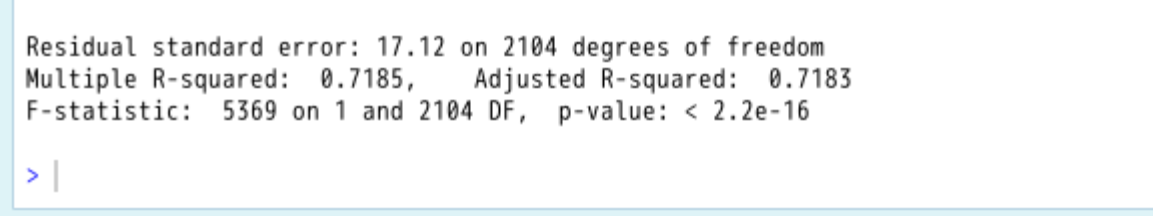
\includegraphics[width=\textwidth]{模型精度-R2}
	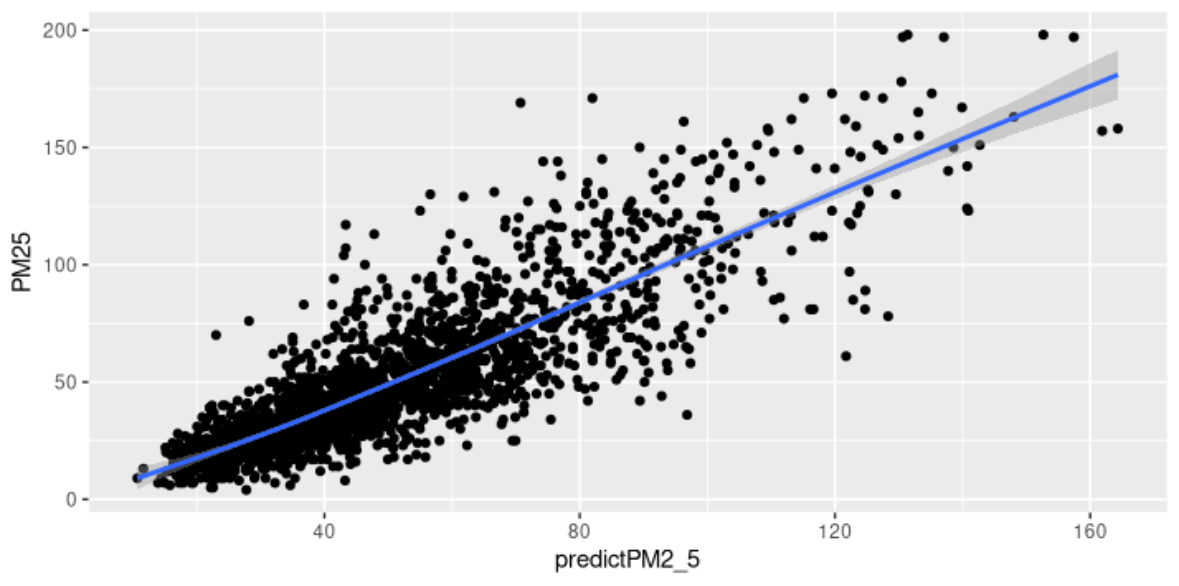
\includegraphics[width=\textwidth]{模型精度}
\end{frame}
\section{介绍}
\begin{frame}{运算流程}
	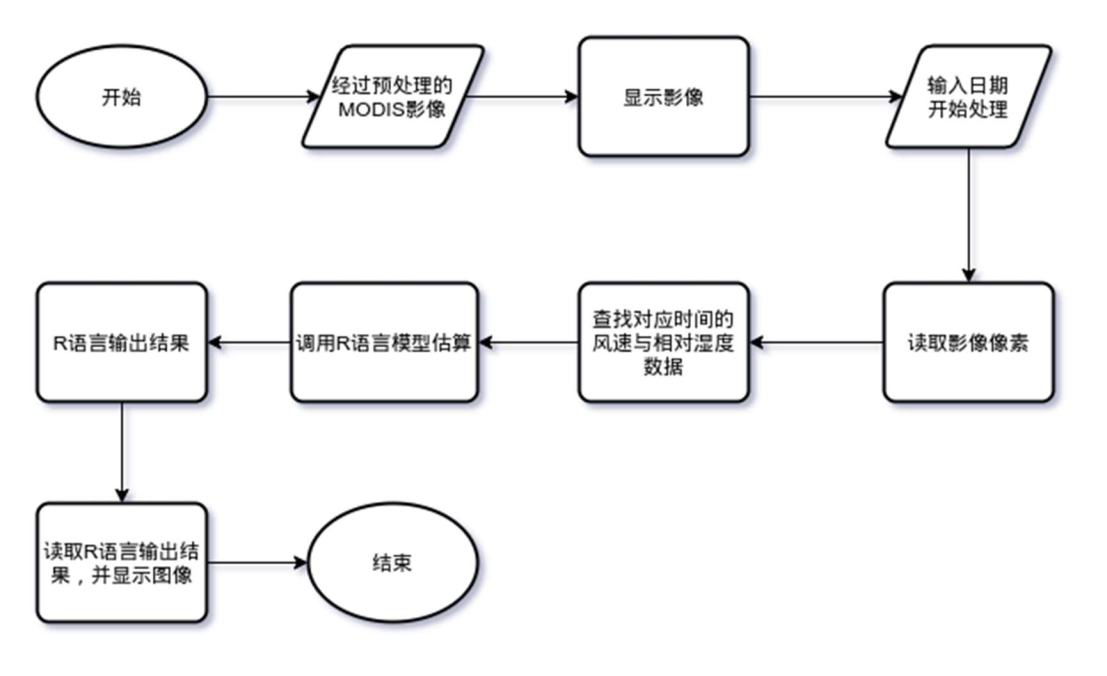
\includegraphics[width=\textwidth]{运行流程}
\end{frame}
\begin{frame}{优势与不足}
	\begin{block}{优势}
		\begin{itemize}
			\item 跨平台
			\item 易分发
		\end{itemize}
	\end{block}
	\begin{block}{不足}
		\begin{itemize}
			\item 功能单一
			\item 速度较慢
		\end{itemize}
	\end{block}
\end{frame}
\begin{frame}{贴图展示}
	\begin{columns}
		\column{.5\textwidth}
		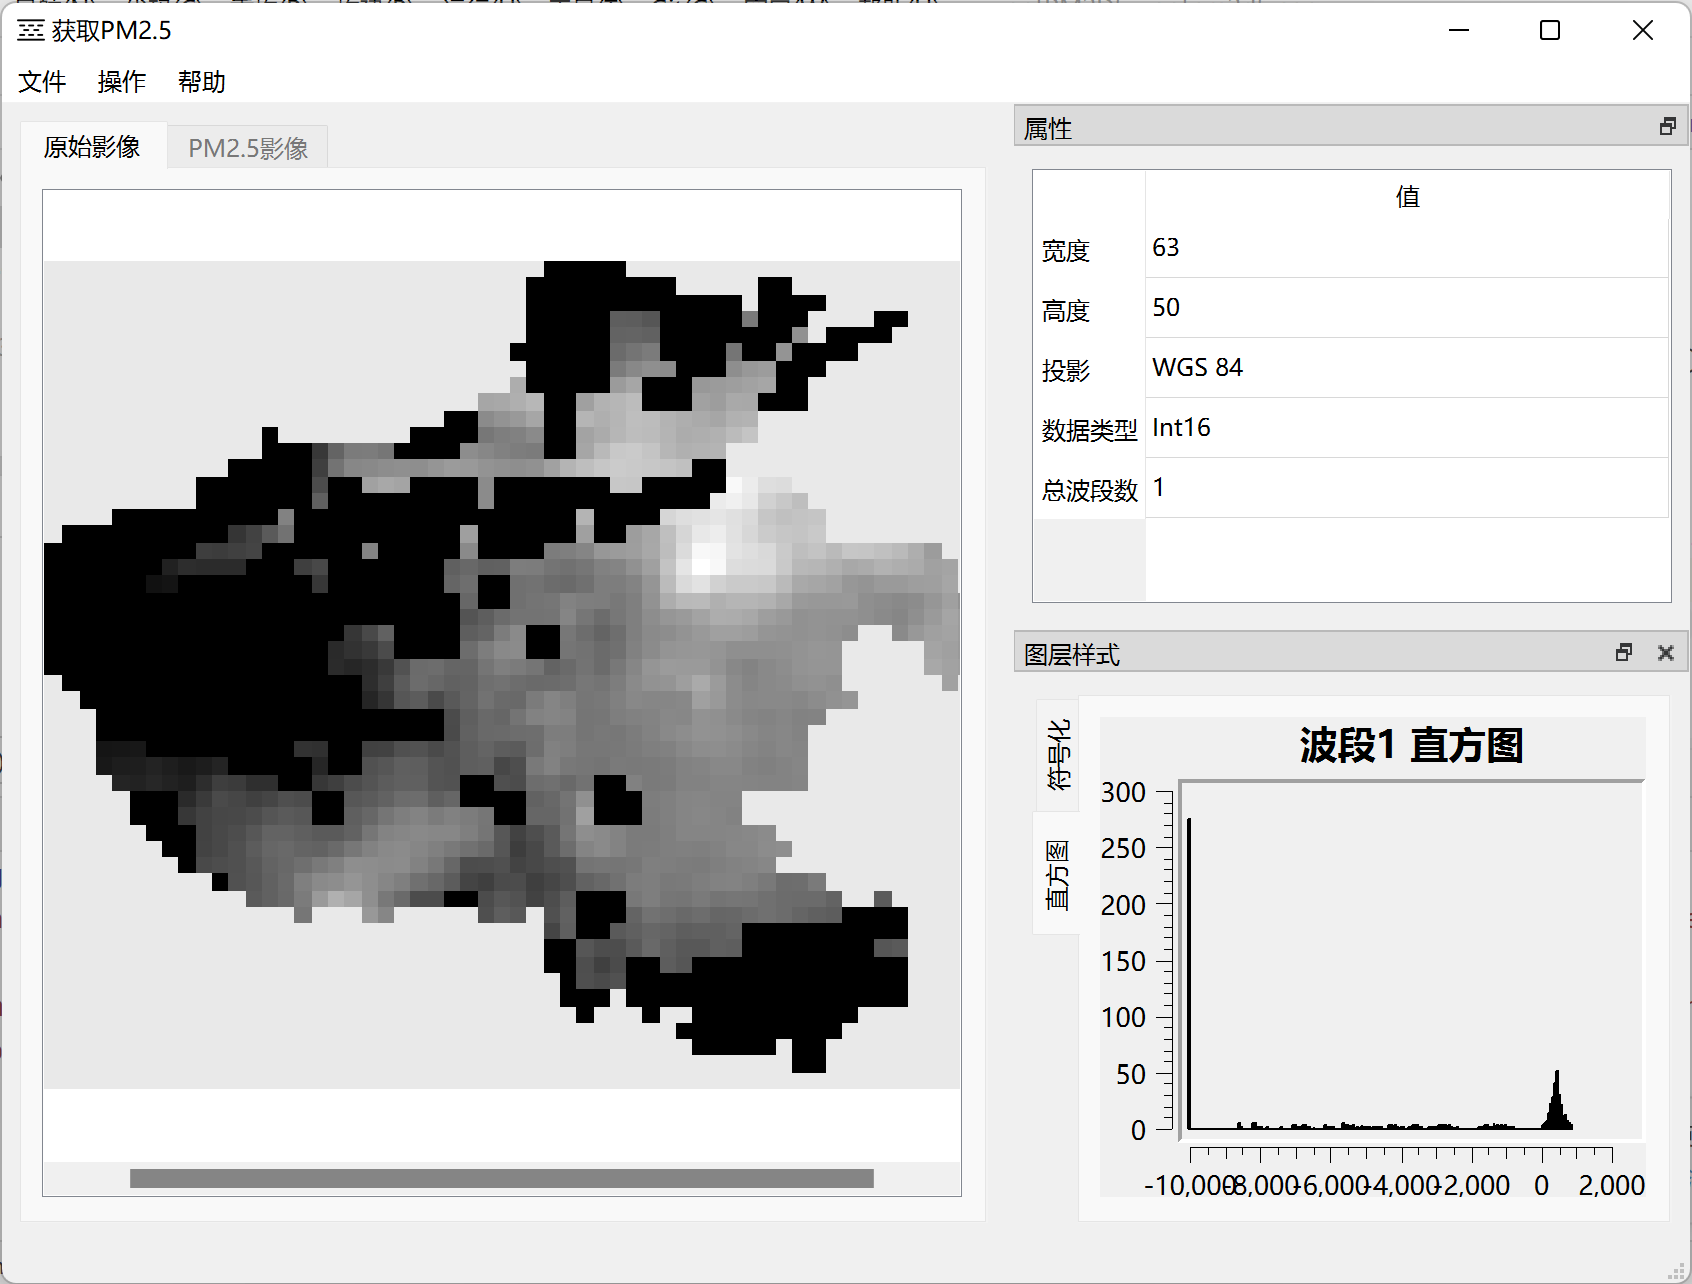
\includegraphics[width=\columnwidth]{getPM2.5程序-打开AOD图像}
		\begin{center}
			打开AOD图像
		\end{center}
		\column{.5\textwidth}
		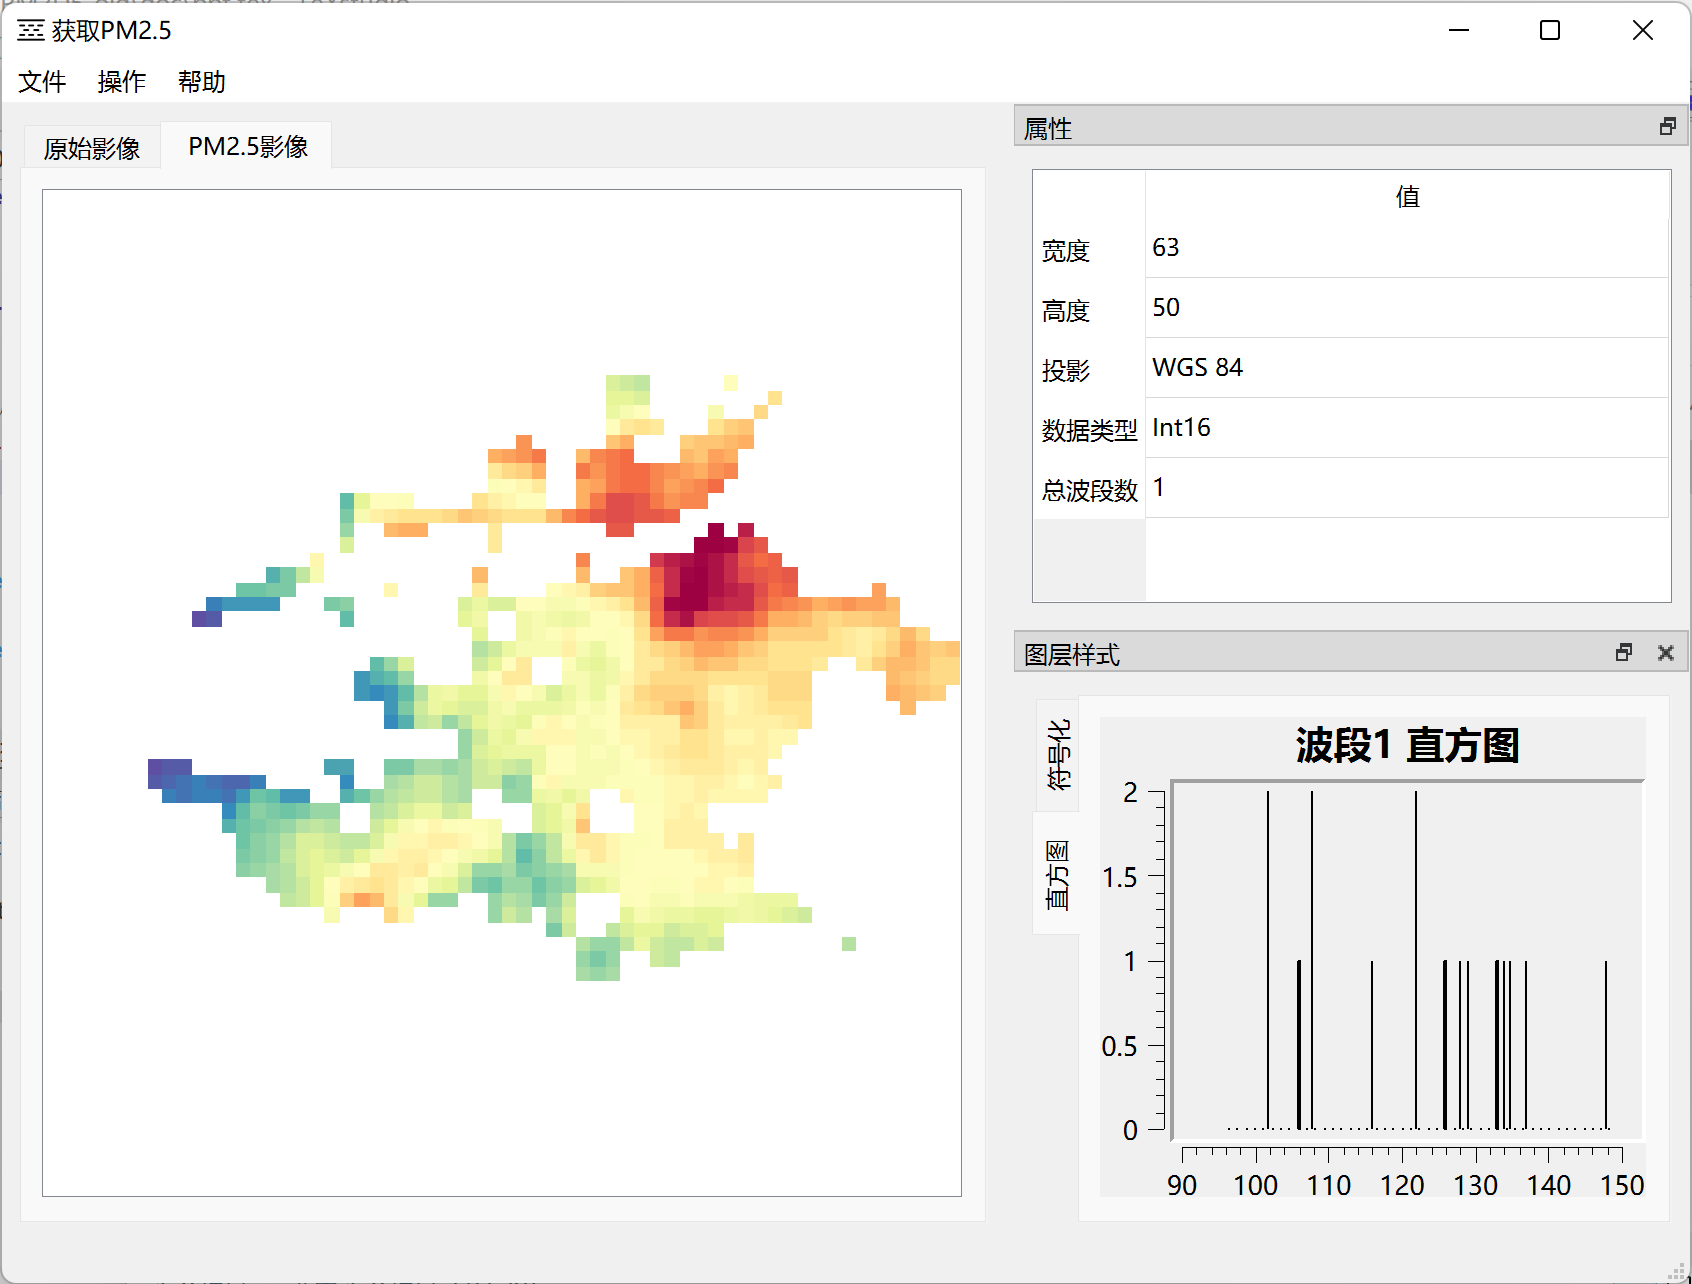
\includegraphics[width=\columnwidth]{getPM2.5程序-渲染PM2.5图像}
		\begin{center}
			渲染PM2.5图像
		\end{center}
	\end{columns}
\end{frame}
\section{演示}
\frame{\frametitle{演示}\centering 实际操作演示}
\section{结束}
\frame{\frametitle{结束}\centering 请老师和同学们批评指教}
\end{document}
